\documentclass{article}

\usepackage{amsmath, amsfonts, listings, amsthm, mathtools, graphicx, pgfplots, tikz, caption, draftwatermark, xcolor, todonotes, listings, color}%pythontex
\setlength\parindent{12pt}
\SetWatermarkText{DRAFT}
\SetWatermarkScale{1}


\newtheorem{theorem}{Theorem}[section]
\newtheorem*{state}{Statement}
\newtheorem{defn}{Definition}[section]

\definecolor{codegreen}{rgb}{0,0.6,0}
\definecolor{codegray}{rgb}{0.5,0.5,0.5}
\definecolor{codepurple}{rgb}{0.58,0,0.82}
\definecolor{backcolour}{rgb}{0.95,0.95,0.92}
 
\lstdefinestyle{mystyle}{
    backgroundcolor=\color{backcolour},   
    commentstyle=\color{codegreen},
    keywordstyle=\color{magenta},
    numberstyle=\tiny\color{codegray},
    stringstyle=\color{codepurple},
    basicstyle=\footnotesize,
    breakatwhitespace=false,         
    breaklines=true,                 
    captionpos=b,                    
    keepspaces=true,                 
    % numbers=left,    
    numbersep=5pt,                  
    showspaces=false,                
    showstringspaces=false,
    showtabs=false,                  
    tabsize=2
}
 
\lstset{style=mystyle}
 

\title{Eulerian Trails and Tours}
\author{Joseph Willard}


\begin{document}
\maketitle


\section{Introduction}
This post discusses the idea behind Eulerian trails and tours. The first section provides some historical insight into the topics as well as a description of the algorithm and related theorems complete with proof. The second section gives python code that simulates finding trails or tours and an explanation behind the process.


\section{Eulerian Trails and Tours}
% discuss algorithm
% discuss BFS
% discuss connected graphs

\subsection{Definitions}

\begin{defn}
Given a graph $G$ the \textbf{degree} of a vertex is the number of edges that touch the vertex. In figure $1$ vertex $E$ on the left graph has a degree of $4$, this is often simplified as $\deg(E) = 4$.
\end{defn}

\begin{defn}
  Given a graph $G$, a \textbf{\textit{walk}} is an alternating sequence of vertices and edges $<v_{0},e_{1},v_{1},\cdots ,e_{n},v_{n}>$. A walk is considered \textbf{\textit{closed}} if $v_{0} = v_{n}$.
\end{defn}

\begin{defn}
A graph $G$ is \textbf{connected} if there exists a walk from any two vertices in $G$.
\end{defn}


\begin{defn}
  A walk is called a \textbf{\textit{trail}} if no edges are repeated.
\end{defn}

\begin{defn}
A graph $G$ has an \textbf{\textit{Eulerian Trail}} if there exists a walk using every edge (see figure $1$). 
\end{defn}

\begin{defn}
A graph $G$ has an \textbf{\textit{Eulerian Tour}} if there exists a \underline{closed} walk using every edge (see figure $1$). 
\end{defn}

\vspace{6cm}

\begin{figure}
\begin{center}
  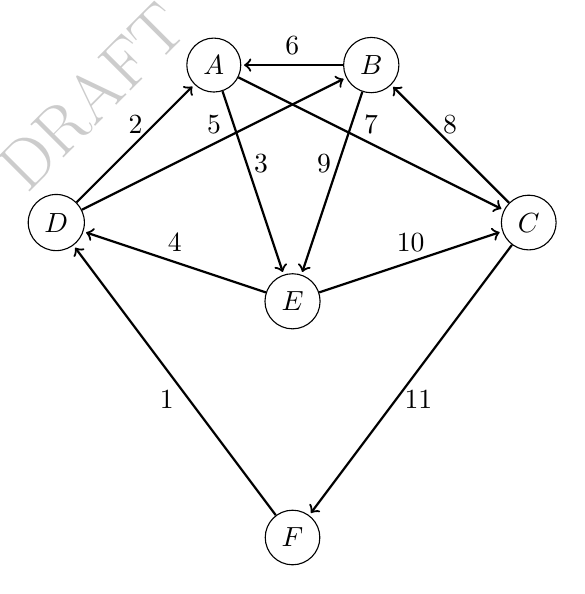
\begin{tikzpicture}[shorten >=1pt,node distance=3cm,auto]
      \node[shape=circle,draw=black] (A)  at (0,0) {$A$};
      \node[shape=circle,draw=black] (B)  at (2,0) {$B$};
      \node[shape=circle,draw=black] (C)  at (4,-2) {$C$};
      \node[shape=circle,draw=black] (D)  at (-2,-2) {$D$};
      \node[shape=circle,draw=black] (E)  at (1,-3) {$E$};
      \node[shape=circle,draw=black] (F)  at (1,-6) {$F$};
      \path[->,draw,thick]
      (F) edge node[below, xshift=-1mm] {$1$} (D)
      (D) edge node[above] {$2$} (A)
      (A) edge node[above, xshift=1mm] {$3$} (E)
      (E) edge node[above] {$4$} (D)
      (D) edge node[above] {$5$} (B)
      (B) edge node[above] {$6$} (A)
      (A) edge node[above] {$7$} (C)
      (C) edge node[above] {$8$} (B)
      (B) edge node[above,xshift=-1mm] {$9$} (E)
      (E) edge node[above] {$10$} (C)
      (C) edge node[below, xshift=1mm] {$11$} (F);
    \end{tikzpicture}
%\caption{Eulerian Tour} \label{fig:Eulerian Tour}
\qquad
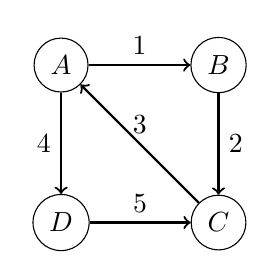
\begin{tikzpicture}
      \node[shape=circle,draw=black] (A)  at (0,0) {$A$};
      \node[shape=circle,draw=black] (B)  at (2,0) {$B$};
      \node[shape=circle,draw=black] (C)  at (2,-2) {$C$};
      \node[shape=circle,draw=black] (D)  at (0,-2) {$D$};
      \path[->,draw,thick]
      (A) edge node[above] {$1$} (B)
      (B) edge node[right] {$2$} (C)
      (C) edge node[above] {$3$} (A)
      (A) edge node[left] {$4$} (D)
      (D) edge node[above] {$5$} (C);
\end{tikzpicture}
%\caption{Eulerian Trail} \label{fig:Eulerian Trail}
\end{center}
\caption{Eulerian Tour (left) and Eulerian Trail (right)} \label{fig:Eulerian Trail}
\end{figure}

\subsection{History}
Historically the idea of of an Eulerian Tour/Trail can be linked back to the Seven Bridges of K{\"o}nigsberg (see figure $2$), which was at the time a city in Prussia but now located in Russia. The question involves finding a way to cross each bridge only once. Euler reformulated the question such that it relied on the number of bridge crossings, labelling the land masses as nodes. This allowed him to make generalize that to use every bridge in a graph there must either exist all even degree vertices or exactly two (see below for proof).
\begin{figure}
  \begin{center}
    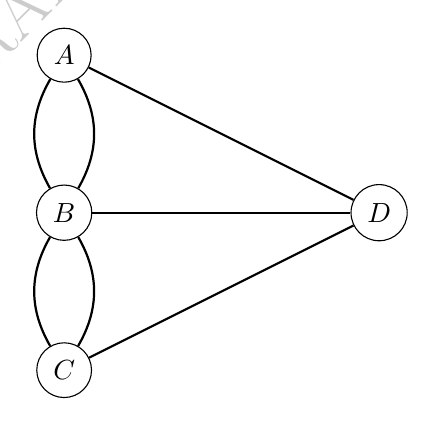
\begin{tikzpicture}
      \node[shape=circle,draw=black] (A)  at (0,0) {$A$};
      \node[shape=circle,draw=black] (B)  at (0,-2) {$B$};
      \node[shape=circle,draw=black] (C)  at (0,-4) {$C$};
      \node[shape=circle,draw=black] (D)  at (4,-2) {$D$};
      \path[draw, thick]
      (A) edge (D)
      (B) edge (D)
      (C) edge (D)
      (A) edge[bend right] (B)
      (B) edge[bend right] (A)
      (C) edge[bend right] (B)
      (B) edge[bend right] (C);
    \end{tikzpicture}
  \end{center}
\caption{Bridges of K{\"o}nigsberg, the nodes are islands and the edges are bridges.}
\end{figure}

\vspace{10cm}
\subsection{Theorems}

\begin{theorem}
If $G$ is a connected finite graph with every vertex having even degree, then $G$ has an Eulerian Tour.
\end{theorem}

\begin{proof}
  Before addressing this it is important to address the case when a graph $G$ has no edges. In this case then there trivially exists an Eulerian Tour since there exists no edges to use. In the case where $G$ is connected arbitrarily choose a starting vertex $v_{0}$. since it is given that each vertex of $G$ is even the when moving from $v_{0}$ to an adjacent vertex $v_{1}$ both have an odd number of unused edges incident to them respectively. Continue this process and every time an unused edge is chosen the incident vertices will have an even number of unused edges except the $v_{0}$. continue doing this until the starting vertex is reached, which is possible because $G$ is connected and every vertex except $v_{0}$ must have an unused edge to leave with.

  If all edges are used in this process then the resulting path gives an Eulerian Tour. If there still exists unused edges then starting from an incident vertex repeat the same process which is again possible since $G$ is connected and in the from the first iteration of this process we used an even number of edges hence each vertex should still have an even degree.
\end{proof}


\begin{theorem}
If $G$ is a connected finite graph with exactly two vertices of odd degree $v$ and $u$, then there is an Euleria Trail starting from $v$ and ending at $u$ (same can be said by starting at $u$ and ending at $v$).
\end{theorem}


\begin{proof}
  Without loss of generality starting at vertex $v$ start creating a path always choosing an unused edge. Continue this process until a vertex is reached that has no unsused edges to leave by. Since every vertex except $u$ and $v$ must have even degree when we approach any of these vertices there is an edge to leave with, furthermore, by starting at $v$ only one edge was used to leave hence it has an even amount of unused edges. Putting all these observations together it is clear that the only possible vertex to get stuck at must be one with an odd degree which is $u$.

  If all edges were used in this process then the output will be an Eulerian Trail. However, if there remains unused edges then they must have even degree, since $u$ is the only possible vertex to get stuck at. From these unused vertices create another path and append it to the originall creating an Eulerian Trail.
\end{proof}


\section{Code}


\begin{lstlisting}[language=Python]
'''
This takes input in the form of tuples (see the bottom of program for example) representing edges of a graph and determines whether they form either an Eulerian trail/tour. If they do it returns the edges in the respective order.
'''


import networkx as nx
import matplotlib.pyplot as plt
import ast as a



edges_input = input("Please enter edges as tuples followed by a comma (e.x, (1,2), (2,3), ... ): ")
edges = a.literal_eval(edges_input)
vertices = int(input("How many vertices in total? "))


def degrees():
    """
    This determines the degree of each respective vertex.
    """
    a = edges
    b = []
    odd = []
    zeroes = []
    
    for i in range(vertices):
        c = 0
        for j in range(len(edges)):
            if i+1 == a[j][0]: 
                c += 1
            if i+1 == a[j][1]:
                c += 1
        b.append(c)
    for i in range(vertices):
        if b[i]%2 != 0:
            odd.append(i+1)
    for i in range(vertices):
        if b[i] == 0:
            zeroes.append(i+1)

    return b, odd, zeroes

def connected():
    """
    This determines whether the graph is connected by performing a breadth first search.
    """
    
    
    b = list(edges)
    path = []
    vertices_travelled = [b[0][0]]
    f = 0
    
    while f < vertices + 1:    
        for i in range(len(b)):
            if b[i][0] not in vertices_travelled and b[i][1] in vertices_travelled:
                vertices_travelled.append(b[i][0])
                path.append(b[i])
            elif b[i][1] not in vertices_travelled and b[i][0] in vertices_travelled:
                vertices_travelled.append(b[i][1])
                path.append(b[i])
            elif b[i][1] in vertices_travelled and b[i][0] in vertices_travelled:
                path.append(b[i])
            elif b[i][1] not in vertices_travelled and b[i][0] not in vertices_travelled:
                pass
        f += 1
        b = list(set(b) - set(path))
            
    return  vertices_travelled, b


    

def euler_trail(x):
    """
    This chooses one of the odd degree vertices and builds a path starting from there.
    """
    b = list(x)
    a = degrees()[1][0]
    path = []
    
    for i in range(len(x)): 
        for i in range(len(b)):
            if b[i][0] == a:
                path.append(b[i])
                a = b[i][1]
                
            elif b[i][1] == a:
                path.append(b[i])
                a = b[i][0]

        for i in range(len(path)):
            if path[i] in b:
                del b[b.index(path[i])]
                
        
        
    return path, b

def euler_tour(x):
    """
    This chooses the first available vertex and builds a path starting from there by always choosing an unused edge.
    """
    b = list(x)
    a = b[0][0]
    path = []
    y = 0

    for y in range(len(x)): 
        for i in range(len(b)):
            if b[i][0] == a:
                path.append(b[i])
                a = b[i][1]
                
            elif b[i][1] == a:
                path.append(b[i])
                a = b[i][0]

        for j in range(len(path)):
            if path[j] in b:
                del b[b.index(path[j])]
        
        
    return path, b



        
    
def cpath(x):
    """
    This function takes the unused edges from either euler_trail or euler_tour and makes a new path.
    """
    opath = x[0]
    b = x[1]
    a = b[0][0]
    path = []
    y = vertices
    i = 0
    
   
    while True:
        if len(b) > 0:
            if i < len(b):
                while True: 
                    if b[i][0] == a:
                        path.append(b[i])
                        a = b[i][1]
                        del b[i]
                        i = 0
                        break
                
                    elif b[i][1] == a:
                        path.append(b[i])
                        a = b[i][0]
                        del b[i]
                        i = 0
                        break

                    else:
                        y = y - 1
                        i += 1
                        break
            else:
                break
                

        else:
            break
            

            
            
            
                    
            
    return opath, path, b



    
def add(x):
    """
    This takes trails from the cpath and finds a place to append them in the trail created by either euler_tour or euler_trail.
    """
    fpath = []
    npath = x[0]
    path = x[1]
    z = x[2]
    c = 0

    while True:
        if len(z) > 0:
            fpath = []
        
            while True: #c < len(x[0]) + 1:
            
        
                if path[0][0] in npath[c] and path[-1][0] in npath[c+1]:
                    npath.insert(c+1, path)
                    break
                elif path[0][0] in npath[c] and path[-1][1] in npath[c+1]:
                    npath.insert(c+1, path)
                    break
                elif path[0][1] in npath[c] and path[-1][0] in npath[c+1]:
                    npath.insert(c+1, path)
                    break
                elif path[0][1] in npath[c] and path[-1][1] in npath[c+1]:
                    npath.insert(c+1, path)
                    break
                c += 1     

            for i in range(len(npath)):
                if type(npath[i]) == list:
                    for j in range(len(npath[i])):
                        fpath.append(npath[i][j])
                else:
                    fpath.append(npath[i])
                    
            npath = fpath
            new_path = cpath((npath, z))
            path = new_path[1]
            z = new_path[2]
            c = 0
            

        elif len(z) == 0 and len(path) > 0:
            fpath = []
        
            while True: 
            
        
                if path[0][0] in npath[c] and path[-1][0] in npath[c+1]:
                    npath.insert(c+1, path)
                    break
                elif path[0][0] in npath[c] and path[-1][1] in npath[c+1]:
                    npath.insert(c+1, path)
                    break
                elif path[0][1] in npath[c] and path[-1][0] in npath[c+1]:
                    npath.insert(c+1, path)
                    break
                elif path[0][1] in npath[c] and path[-1][1] in npath[c+1]:
                    npath.insert(c+1, path)
                    break
                c += 1     

            for i in range(len(npath)):
                if type(npath[i]) == list:
                    for j in range(len(npath[i])):
                        fpath.append(npath[i][j])
                else:
                    fpath.append(npath[i])
                    
            npath = fpath
                
                
            c = 0
            break
        else:
            break
                    

    return npath, z

    
def clean(x):
    """
    This takes the input and arranges the tuples so that the final output gives a walk to follow (i.e (1,2), (2,3), ...etc).
    """
    path = x[0]
    clean = [path[0]]

    for i in range(len(path) - 1):
        if clean[i][1] == path[i+1][0]:
            clean.append(path[i+1])
        else:
            clean.append((path[i+1][1], path[i+1][0]))

    return clean


    

def trail(x):
    """
    This fucntions purpose is to give the correct output of the program taking into account whether the input is connected and has the correct number of odd degree vertices.
    """
    
    if len(connected()[0]) != vertices:
        return "This graph is not connected!"
    
    elif len(degrees()[1]) == 2 and len(euler_trail(x)[1]) == 0:
        return  "The Eulerian Trail is: ", clean(euler_trail(x))
    
    elif len(degrees()[1]) == 2 and len(euler_trail(x)[1]) != 0:
        return "The Eulerian Trail is: ", clean(add(cpath(euler_trail(x))))
                                                 
    elif len(degrees()[1]) == 0 and len(euler_tour(x)[1]) != 0:
        return "The Eulerian Tour is: ", clean(add(cpath(euler_tour(x))))
                                                 
    elif len(degrees()[1]) == 0:
        return "The Eulerian Tour is: ", clean(euler_tour(x))
                                                 
    else:
        return "there exists neither an Eulerian Tour or Trail due to the number of odd degree vertices."

G = nx.Graph(list(edges))
nx.draw(G)
plt.show()
print(trail(edges))



        



#5 ,(1, 2), (2, 4), (5, 1), (2, 3), (5, 4), (2, 3), (4, 1), (1, 3), trail

#10 (1, 2), (4, 4), (2, 4), (7, 8), (5, 1), (8, 9), (2, 3), (6, 8), (5, 4), (7, 8), (2, 3), (10, 9), (4, 1), (6, 10), (1, 3), not connected 

#14, (1, 2), (9, 11), (4, 4), (3, 14), (2, 4), (5, 11), (7, 8), (5, 1), (11, 13), (8, 9), (5, 13), (2, 3), (14, 11), (6, 8), (13, 2), (5, 4), (7, 8), (9, 14), (2, 3), (10, 9), (4, 1), (13, 2), (6, 10), (1, 3), not connected since 12 is never reached.

#16, (1, 2), (9, 11), (4, 4), (3, 14), (2, 4), (15, 12), (6, 9), (5, 11), (7, 8), (5, 1), (11, 13), (8, 9), (5, 13), (2, 3), (14, 11), (6, 8), (13, 2), (5, 4), (16, 1), (7, 8), (15, 6), (9, 14), (11, 16), (2, 3), (15, 2), (4, 12), (10, 9), (4, 1), (13, 2), (6, 10), (1, 3) Too many odd.

#18, (1, 2), (9, 11), (4, 4), (17, 16), (3, 14), (16, 15), (2, 4), (15, 12), (6, 9), (13, 13), (5, 11), (7, 8),  (17, 11),  (2, 14), (5, 1), (11, 13), (8, 9), (5, 13), (2, 3), (1, 18), (14, 11), (6, 8), (13, 2),(5, 4), (18, 9), (16, 1), (7, 8), (15, 6), (9, 14), (11, 16), (2, 3), (15, 2), (4, 12), (10, 9), (4, 1), (13, 2), (6, 10), (1, 3) tour

#15, (1, 2), (1, 3), (1, 4), (2, 3), (4, 5), (4, 6), (4, 7), (5, 8), (5, 9), (5, 10), (6, 7), (8, 9), (10, 11), (10, 12), (10, 13), (11, 14), (11, 15), (12, 13), (14, 15) trail
\end{lstlisting}







\end{document}